\section{Introduction}

SDN is an evolved networking paradigm which has changed the way a network operates when compared to conventional networks. A traditional network uses different set of devices like router and switches to provide connectivity to the entire network. A set of forwarding rules in these devices decide and direct the flow of a network traffic. Network admin, generally is responsible to program and maintain these forwarding 
rules individually in all switches and routers. Control plane on each device
keeps track of forwarding logic and instructs the forwarding plane\footnote
{Also called Data Plane} to make routing decisions. 
Software-Defined Networking has brought significant change as networks function by
decoupling the entire control plane from the every device in a forwarding plane. Abstraction of higher level functionality is thus achieved and the intelligence of entire 
network  is now moved to a centralized location called SDN-Controller. 
Result of this new architecture with central programmability and visibility is tremendous improvements in operational cost and ease in maintenance.

Reaping advantages have influenced both industries and academic institutions to  persistently work towards adaptation and evolution of SDN networks. The strong push of cost effective scalable networks has lead to transformation of traditional networks and deployment of SDN infrastructure in production networks like Data-Centers and enterprise Clouds. Growing merits of SDN have also made it increasingly popular among academic institutions. The campus networks today generate tremendous amount of traffic making data intensive science a common norm.
To appropriately handle data without significant loss in information, campus networks have begin to dedicate a portion of their network model for advanced research operations.

This new model termed as Science-DMZ \cite{SCIENCEDMZ}, is a SDN based solution specifically designed for optimizing network transactions on academic networks. The model allows for existing tools and methods to be optimized for protecting science critical systems.
Science-DMZ is often built around the campus' local network perimeter. To employ a belt of security in this perimeter network, institutions often depend on legacy firewalls and Intrusion Detection Systems. However, both of these security mechanisms are ill-suited for protecting SDN environments. Traditional firewall functions are based on static rule set consisting of \textit{allow} or \textit{deny} policies. Filtering
of network traffic is done by matching every packet against these policies. Most of the granular rules can match a packet against only source and destination IP addresses and TCP/UDP ports. These kind of rules cannot be further fine grained and therefore, lack adaptivity and scalability. Consequently, an SDN-Firewall solution is vital to work closely with the SDN-Controller and take advantage of the centralized view of entire network.

Some related work has been done in the recent past to address security concerns specific to SDN networks. There also exist SDN based firewalls
which work in collaboration with controller and provide centralized security framework. However, these firewall solutions are often presented as a prototype intended to work on small-scale controllers with dated versions of OpenFlow protocol. Additionally, they often employ network simulation techniques like mininet\cite{MININET} for their evaluation. These firewall designs face challenges in adapting to rapidly evolving SDN controllers' designs and revisions in OpenFlow. Thus, there lies an inherent need of revisiting the SDN firewalls to discover underlying shortcomings which are result of deploying them over a more real-time and large-scale network.

In this paper, we have revisited existing SDN-based firewall designs to asses their readiness to protect a large scale SDN deployment. Additionally, an attempt to revamp one of these firewall designs\cite{FLOWGUARD} to work closely with the mainstream SDN controller, OpenDayLight, has been made. The underlying network, ScienceDMZ\cite{SCIENCEDMZ} which is used for experiments is more realtime than a simulation \cite{MININET}. 
It is thereby observed that the proposed approaches to detect policy violations are prone to security loopholes that urgently need to get addressed for promised SDN security. It is also discovered that the defense and attack mitigation models are obsolete and incomplete to safeguard a larger network with various changes in controller design. Vulnerabilities found in existing solutions are investigated and suitable defense mechanisms, when applicable, are also proposed. Finally, it is shown that performance of present SDN firewalls (tested only in simulated environments) is unfit in terms of feasibility on an enterprise network: we have identified a room for improvement by proposing a modified algorithm to detect policy violation. 

\section{SDN Background}
\subsection{Openflow}
Communications between SDN logical abstractions is achieved by using different protocols depending on the layers wanting to communicate. The decoupled control plane logic makes the forwarding decision along with policy enforcement. This information sharing between SDN-Controller and switches takes place using apis provisioned by a southbound OpenFlow protocol.
Controller leverages OpenFlow protocol to pull the information from switches and feed the forwarding logic back. OpenFlow enabled switches maintain the flow routing policies in flow tables. A typical rule present in a flow-table has 3 different field sets for packet handling: Match, Action and Statistics. The match set allows packet filtering based on layer 1-4 header fields. Rules are matched based on priorities and after a successful match, packets undergo respective action present in the rule. According to OpenFlow standard, first packet of every network flow is typically sent to the controller which then inspects the packet headers and decides actions to be taken for rest of the flow. These actions can be either \textit{drop}, \textit{forward} or \textit{send to controller}. The control plane can potentially enforce the centrally stored security policies and take a suitable action for every packet that is received by it. This central visibility is of great advantage as controller can extrapolate the future impact of a traffic on any other node in the network.

\subsection{Controller Design}
SDN-Controllers are capable of a lot more than a traditional control plane where a particular node remains oblivious of network activity in any other node in the network. There are different SDN controllers present in market. Some light weighted ones are used for academic testing and prototyping. The enterprise-ready controllers however are complicated in their design and functioning. Due to lack of implementation standards, these controllers are implemented differently and often leave security loopholes in their implementation and design. Two of the most widely recognized SDN controllers in the market are OpenDayLight \footnote{Henceforth, referred as ODL} and Open Network Operating System\footnote{Henceforth, referred as ONOS}, both are open-source projects hosted by The Linux Foundation \cite{TLF}. They both also differ greatly in their internal designs and implementation. 
\begin{comment}
\subsubsection{OpenDaylight}
OpenDayLight is a SDN controller based on Model-View-Control platform written in Java. ODL provides several controller services implemented as part of it's kernel and Service Abstraction Layer, MD-SAL. Some of the major services running in ODL include L2switch, OpenflowPlugin and MD-SAL. To operate concurrently, these services take data from a common information storehouse present within the ODL core architecture. To store the data coming from northbound REST APIs and from southbound OpenFlow protocol, ODL, implements two logical datastores. Operational store contains the active and opearting state of the network, the information is directly retrieved from the network. Config store, however, contains information as the applications operating on controller and the network administrator intends. This is different from operational store in which it does not retrieve the information from the network. Instead, it contains information  that is directly fed to it using REST APIs and also programmaticaly from services like firewall running inside or outside controller.
Consequently, the administrator or a Firewall application can only make GET requests from the operational datastore. But, the CONFIG datastore provides GET, PUT, POST and DELETE procedural transactions for playing with data. An SDN firewall typically makes GET information to retrieve the latest flow rules and topology of the network. CONFIG store is used by a firewall to put the counter measures and to modify the existing OpenFlow rules. Finally, ODL discourages use of external databases for the performance reasons and leverages its in-memory datastores based on XSQL. 

\subsubsection{Open Network Operating System}

ONOS is being marketed as a SDN Operating System rather than as a controller. Different subsystems on ONOS gives the modularity and high level of service abstraction. Common subsystems on ONOS include Device, Link and FlowRule subsystems. The datastores here are divided in two categories: services running on controller have separate datastore per service and each device present in the network has a datastore of its own. Device and topology information is stored in Device Config Store, implemented using distributed Doctree model. The services like firewall get a separate Service Config Store. Applications can initiate the transfer of config parameters from service to device config store. Device drivers ultimately then program the switches present in the topology.  
\end{comment}
\subsection{Firewalls}
\begin{figure}
	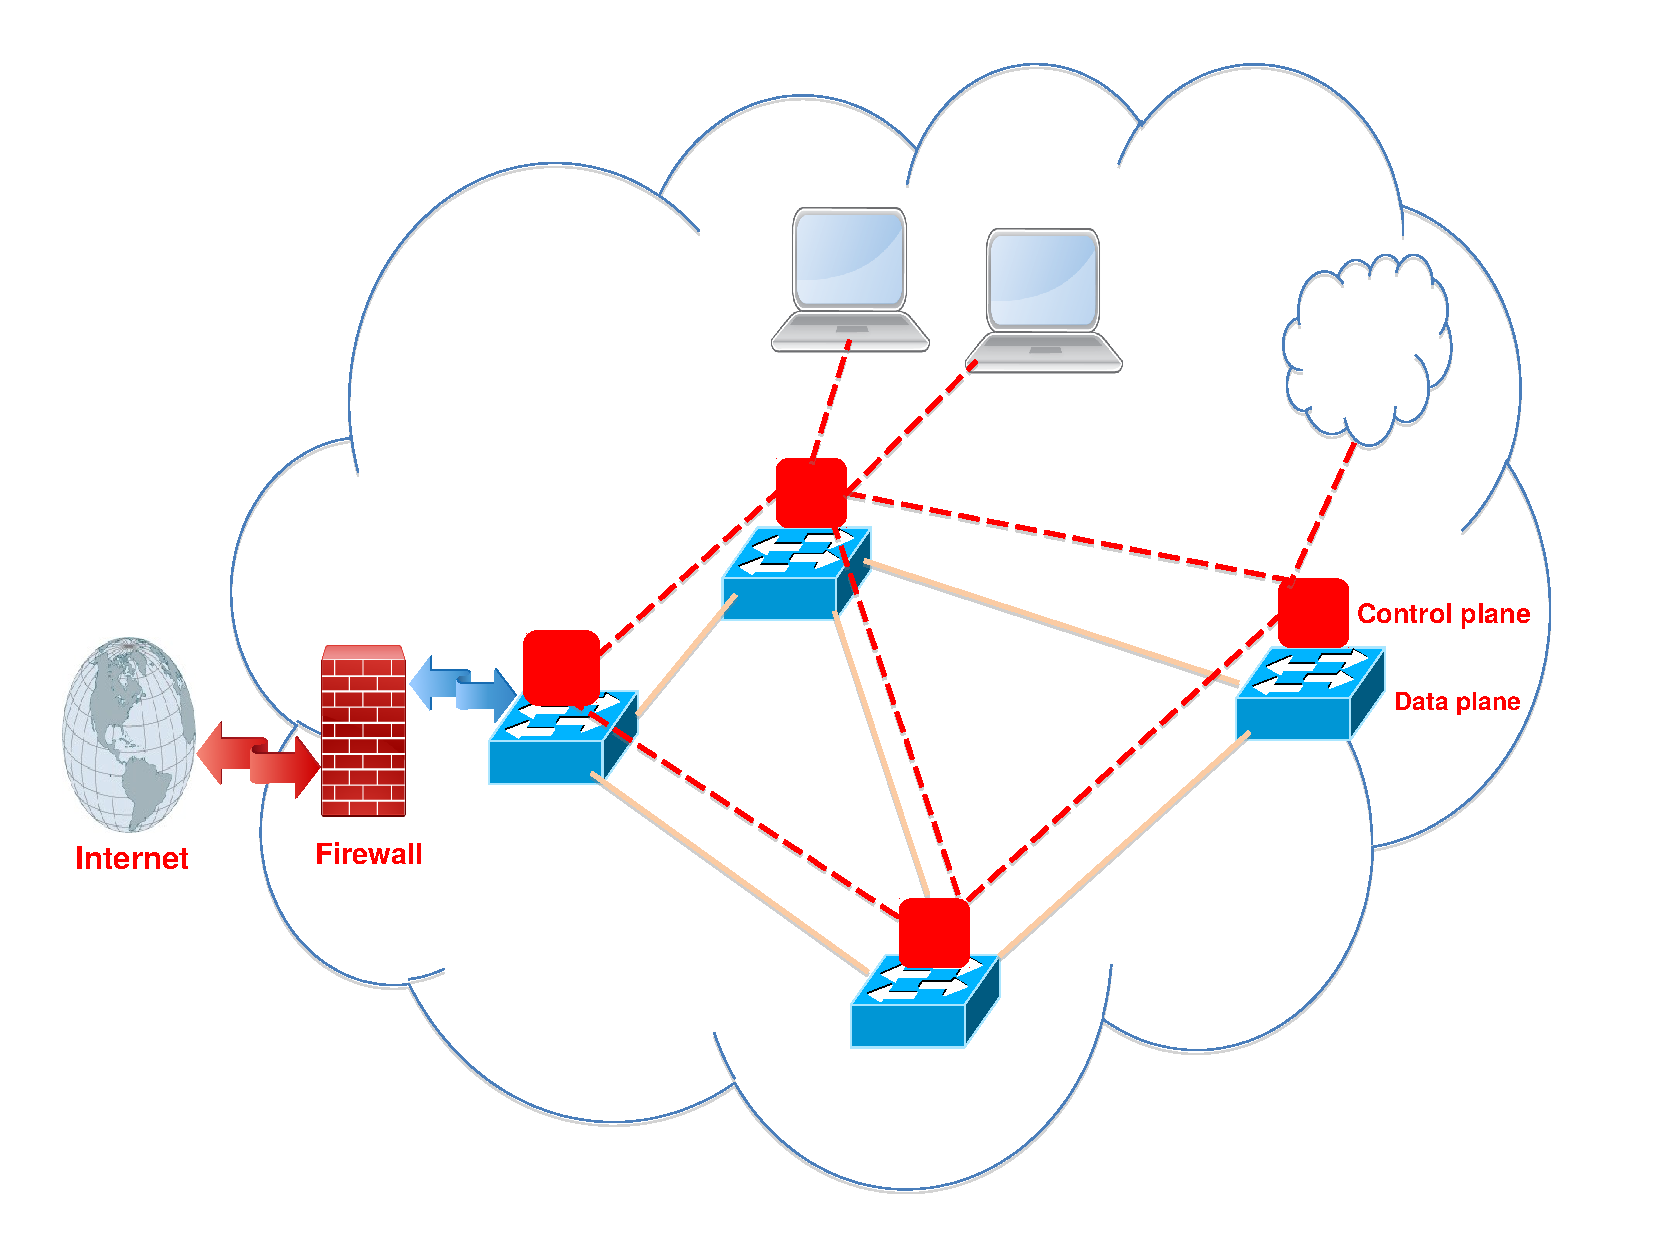
\includegraphics[height=3in, width=3in]{Pictures/traditionalFW.pdf}
	\caption{ Firewall in  \texttt{traditional} network}
	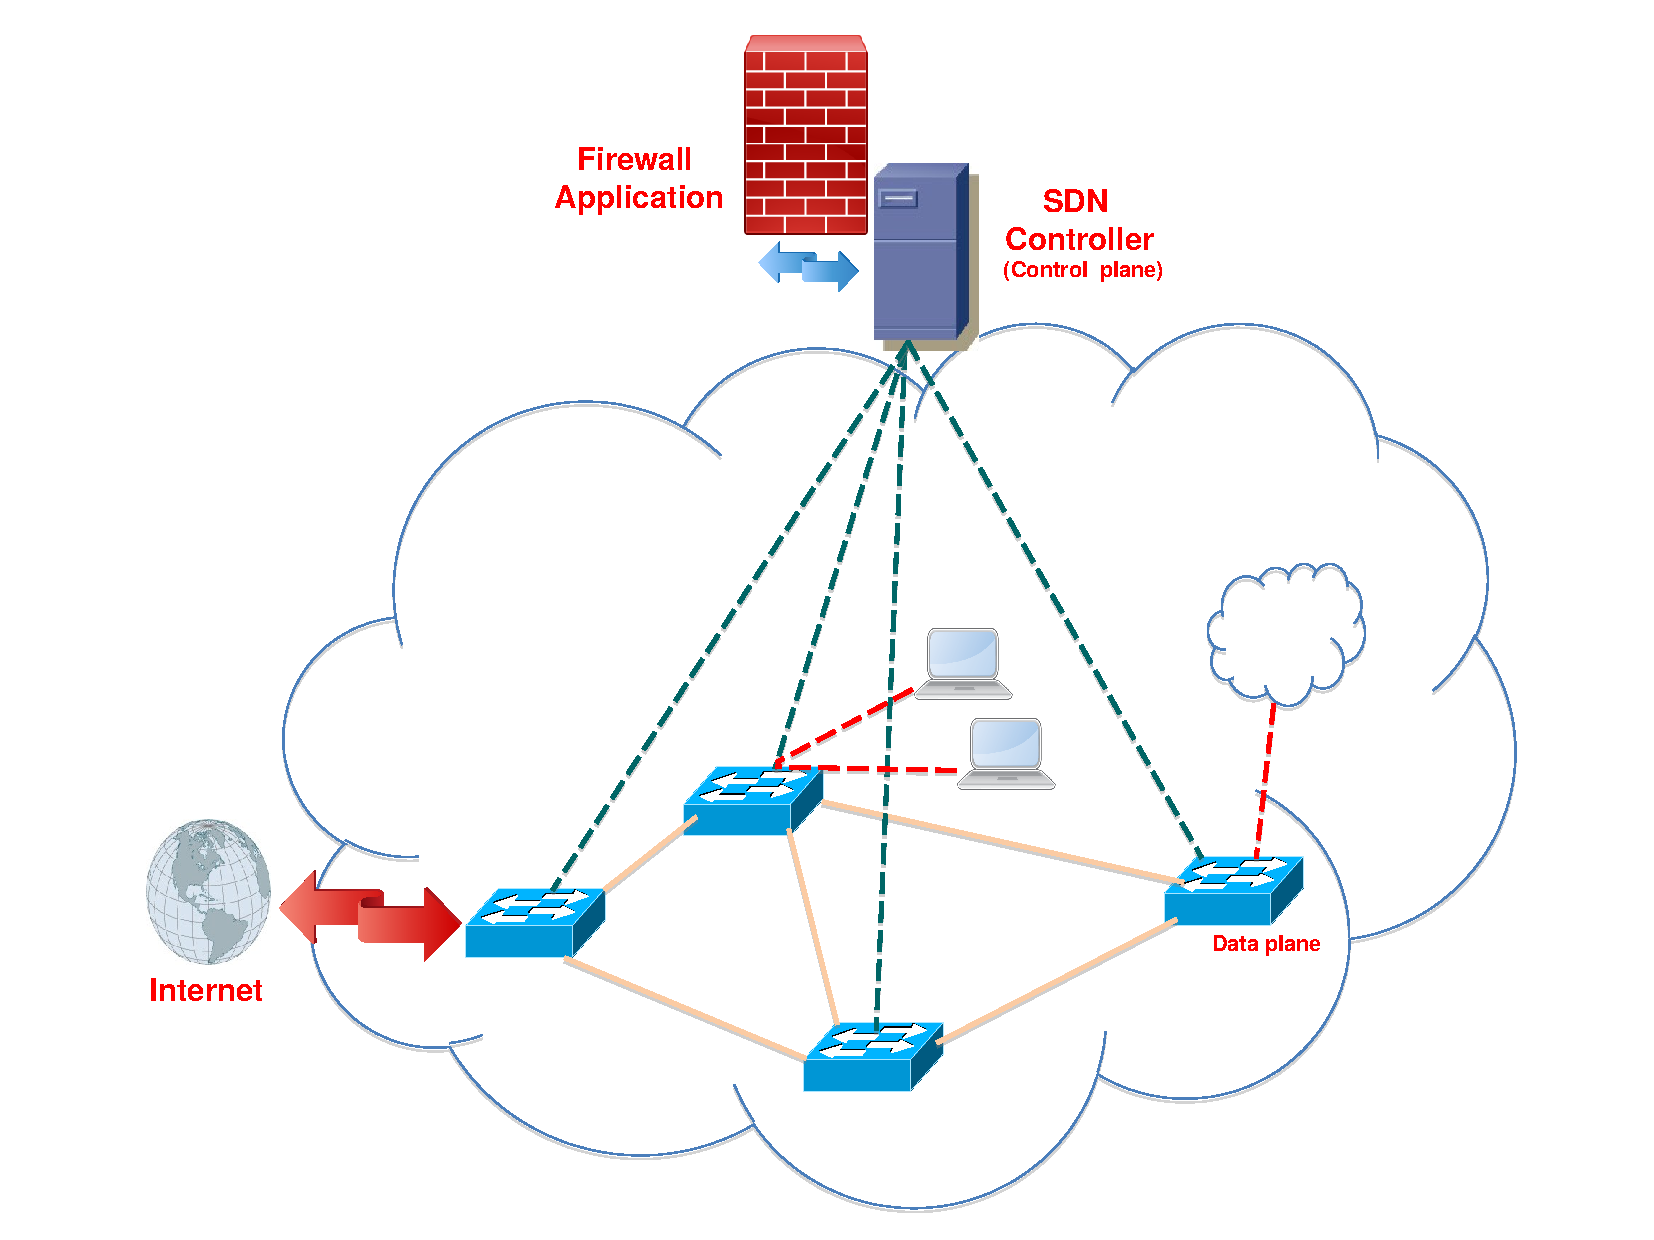
\includegraphics[height=3in, width=3in]{Pictures/SDNFW.pdf}
	\caption{ Firewall in  \texttt{SDN} network}
\end{figure}  
A conventional firewall is a system that protects trusted internal network from the untrusted and unsecured outside world, such as Internet.
Firewalls filter and scan the traffic in and out of the network. Layer-3 and Layer-4 header fields from a traffic flow are compared against a static set of security policies, such as ACLs. In a paradigm of SDN, the positioning, functioning and capabilities of a firewall witness multiple adaptations. SDN architecture allows the network to be managed centrally, deeming the forwarding plane only to be a set of vacuous boxes. The firewall logic should be placed on a control plane alongside the controller and thus demanding a novel design meant to protect an SDN network. Firewall having a centralized view of a network can additionally inspect local traffic to detect internal policy violations and network reachability. The firewall policies are centrally enforced at the controller and a software application is responsible for installing filtering rules on the network.
Unlike traditional firewall which filters and scans every packet coming and going through it, an SDN-Firewall gets the first packet of each flow and installs flow rules for the rest of the flow in tables of respective switches. Flows can directly be installed by an administrator and a privileged application in controller too after sanitation done by a firewall. SDN-firewall should check for policy enforcement by verifying the impact of such changes in the network before a violation can potentially happen. 

Additionally, an SDN firewall works on an abstracted design of network. This is different from a traditional firewall. Thus, SDN-Firewall should check for any threats that can originate from northbound and southbound communication.

\section{SDN Firewall Capabilities}
\begin{enumerate}
	\item \textbf{Policy Enforcement: } 
	The basic functionality of any firewall is to enforce security policies in a network. An SDN firewall is capable of doing this centrally. Thus, a SDN network which uses traditional firewall hardware as a node in the network, is not harnessing the benefits of SDN: Centralization and Programmability. Policies can range from having fine granularity to being largely coarse. To enforce security on a network, firewall converts these policies into flow rules which later get installed in the network.  
	\item \textbf{End to End Flow Path Space: }
	The rules installed in the network direct packets belonging to a particular flow from source to destination. Thus any path taken by packets belonging to a connection go through multiple flows in one or more switches. To effectively enforce the policy, an SDN firewall should keep track of the flow path space. Merely confirming the policy on ingress and egress port of a switch cannot guarantee a successful conflict detection, let alone resolving them. Furthermore, OpenFlow protocol allows "set-field" actions which can change the header space of a packet. Building a flow path space further guarantees to take into account such changes in header fields of an in-route flow. 
	\item \textbf{Conflict Resolution: }
	Upon detecting a violation in the rules when a new policy or a flow rule is being added, a comprehensive firewall should provide a conflict resolution too. Different instances prove that just allowing or denying a network update does not make for a efficient firewall design. A policy violation can happen when flow path space includes a particular switch. But, if there exists another path in the network without a conflicting entity, firewall should dynamically perform resolution to give an updated path. Similarly, the new update may only partially cause a violation. In which case, firewall should dissect the update into allowed and denied sets and process the allowed set. Therefore, for an SDN firewall to be  comprehensive in nature, it is important to provide dynamic conflict resolutions too.    
	\item \textbf{Automatic Priority handling: }
	Multiple different sources update the policies in a network. These include and are not limited to users, administrator and security applications running alongside the SDN firewall. Assigning an authorization level to each source is important to prevent low priority updates to shadow the crucial network policies. Moreover, an intelligent firewall should process these authorization issues automatically and provide a robust user experience.
	\item \textbf{Multi Tenant Support: }
	In a complex network like datacenter, there can easily be more than one sub networks. These subnets can be serving a different tenant each. Handling multiple tenants is not a special concern in a traditional network as the different firewalls are dedicated to each tenant network. However, in SDN, the controller has a centralized view of entire network and firewall is responsible to centrally enforcing the policies. Now, an SDN firewall should be capable of generating a distinction among the networks even if the configuration(IP Tuples) appear same in two disconnected networks.
	\item \textbf{Scalability and Concurrency: }
	In a dynamic and scalable network, the updates in security policies are not sequential. In our testing we have found issues when multiple user threads or applications make concurrent updates on firewall policy or flow policy. In case of conflicting updates, lack of handling the concurrency leads to low priority rule with a different action and a same match being handled before the higher priority rule. For eg. if an admin uses REST call to install a new flow rule in the network but an application at the same time installs a conflicting action on the same match, the decision of unsynchronized firewall depends on which thread is executed before. The issue with concurrent updates becomes a problem when firewall applications are deployed in an enterprise networks where there are multiple pipelines which access and update same data stores.
	\item \textbf{Stateful Support: }
	Maintaining states of the active connections gives a definite advantage to the reliability of a firewall. These connection states can be maintained using information from southbound OpenFlow communication. States' information should be formulated into time-bound flow rules for a network. This provides finer granularity in the rules and more accurate violation detection mechanism.
\end{enumerate}

\begin{table*}
	\caption{Comparison of SDN based Firewalls}
	\label{tab:commands}
	\begin{tabular}{lccccccccc}
		\toprule
		Firewall&Controller&\thead{End to End \\ Flows}& \thead{Dynamic Conflict \\ Detection} &\thead{Multi-Tenant\\ support}& \thead{Auto Priority \\ handling}&\thead {Violation\\ Resolution}&\thead{Concurrent \\updates}&Stateful&Year
		\\
		\midrule
		\\
		Ethane\footnotemark{} \cite{ETHANE}& Ethane& $\times$& \checkmark& $\times$& $\times$& $\times$ & $\times$& $\times$ &2007\\\\
		% http://cs.brown.edu/courses/csci2950-u/s14/papers/Casado07Ethane.pdf
		FortNOX \cite{FORTNOX}& NOX& $\times$& \checkmark& $\times$& \checkmark& $\times$ & $\times$& $\times$ &2012\\\\
		% http://www.csl.sri.com/users/vinod/papers/fortnox.pdf
		Flowguard \cite{FLOWGUARD}& FloodLight& \checkmark& \checkmark& $\times$& $\times$& \checkmark & $\times$& $\times$ &2014 \\\\
		% https://pdfs.semanticscholar.org/2bbf/7ca5c2128427df0c0e98d3a9e728aa009280.pdf
		FW over SDN \cite{FWSDN}& POX& $\times$& \checkmark& $\times$& $\times$& $\times$ & $\times$& $\times$ & 2014 \\ \\
		% http://ieeexplore.ieee.org.ezproxy1.lib.asu.edu/stamp/stamp.jsp?arnumber=6779061
		SE-FloodLight\footnotemark{} \cite{SEFLOOD}& FloodLight& $\times$& \checkmark& $\times$& \checkmark& \checkmark & $\times$& $\times$& 2015 \\\\
		% http://www.csl.sri.com/users/porras/SE-Floodlight.pdf
		AuthFlow \cite{AUTHFLOW}& POX& $\times$& \checkmark& $\times$& $\times$& $\times$ & $\times$& $\times$ & 2016\\\\
		% https://www.gta.ufrj.br/ftp/gta/TechReports/MFD14.pdf
		Reactive stateful FW \cite{REACTIVEFW}& RYU& $\times$& \checkmark& $\times$& $\times$& $\times$ & $\times$& \checkmark & 2016\\\\
		% http://hal.univ-brest.fr/hal-01333445/document
		%	Palo-Alto SDN-FW& OpenDayLight& \checkmark& \checkmark& $\times$& $\times$& \checkmark & $\times$& $\times$ \\
		\bottomrule
	\end{tabular}
\end{table*}

\section{Challenges with SDN Firewalls}
SDN-security has been a hot topic for a few years now. However, this focus came almost after a decade since the inception of Software Defined Networking. The very first \cite{ETHANE} work on security of SDN focused only on implementing access control lists within the SDN controller. As described in 2.3, an SDN firewall has a potential of being a holistic network security solution by leveraging centralization, scalability and abstraction at the control plane. Merely implementing a version of Access Control List \cite{FWOSDN} in SDN does not harness the capabilities of SDN at all. Firewalls taking advantage of SDN are being actively researched. Every work on SDN firewall focuses on certain aspect of SDN security but misses some other important measures. The reason for lack of comprehensive solution should not be just accounted for slow progress in the field of security: SDN controllers have not been standardized as well as the north bound communication mechanism. OpenFlow, which is responsible for controller to network communication has a well maintained standard which is intensely adapting to the new requirements. All these together leaves the developed security solutions become obsolete soon after they are proposed. Another issue which glooms the confidence in SDN firewalls is that the existing systems are developed and tested on prototyping controllers. The efficacy of a firewall in an enterprise sized network often remains undetermined. As a part of our tests, when we deployed firewalls \cite{FLOWGUARD}, \cite{SEFLOOD} on the production level of controller, OpenDayLight\cite{ODL}, the results appeared unfavorable. Existing works on SDN firewalls have been discussed below in detail and also populated in Table.

\footnotetext[4]{ETHANE is a SDN architecture with inbuilt security}
\footnotetext[5]{Conflict resolution is not done for policy violations on the network but between competing controller applications} 

The earliest SDN firewall, \textbf{ETHANE} \cite{ETHANE} came along with the very foundation of SDN architecture. It showcased that security policies instead of defined individually on network entities, can be centrally enforced. No mitigation or threat prevention measures were discussed as the focus was on network programmability. With a lack of standard OpenFlow protocol,the policy enforcement was done only per node basis via the controller.  

With time, the SDN infrastructure popularized and standards were developed for OpenFlow protocol. With increasing adaptation of SDN, security loopholes regularly surfaced with various works focusing on attack detection and mitigation in SDN \cite{SDNSURVEY}. The hardware based firewall solutions were not needed anymore for protecting SDN network. However, the software based firewalls suffered due to lack of standards and right evaluation frameworks.

In \cite{FORTNOX}, security kernel has been proposed for the NOX controller. \textbf{FORTNOX} firewall prevents any unauthorized rule installations by assigning controller applications and users an authorization level. If a new rule is installed, the decision to reject the update depends upon the installer's authorization level. FORTNOX, however, is not a comprehensive SDN firewall solution by the virtue of two primary reasons. First, it lacks accuracy as the rule conflict analysis is done in alias sets. The pairwise comparison ignores the multiple rule dependencies and thus, provides an inaccurate result in a complex network with interdependent flow rules. Secondly, FORTNOX does not provide a fine grained resolution after detecting a conflict. A new rule being installed can be only partially violating the security policy and thus should be dissected for the allowed sets in it. Moreover, FORTNOX kernel is designed as an extension for the NOX controller, which is significantly different from enterprise level of controllers. The scalable controllers like OpenDayLight put forward challenges for the prototyped firewalls when several sources race for installing and modifying rules concurrently.
 
A robust SDN firewall \textbf{FLOWGUARD} is proposed in \cite{FLOWGUARD}. FlowGuard is an SDN-Firewall prototype solution built on FloodLight controller and OpenFlow 1.1. To  detect flow policy violations, the firewall pulls network topology and flow rules from the data plane. It has leveraged Header Space analysis \cite{HSA} and NetPlumber library to build a plumbing graph. This graph is used as a logical snapshot of the network. A flow path space is a tracked space of a packet in the network comprising of initial source and final destination addresses. Flow path space calculation is based on IP 5-Tuple sense: source, destination IP and ports with protocol which in our testing we found being ambiguous in multi-tenant networks. Further, comparing the flow path space against the Firewall DENY rules, FlowGuard detects any security policy violations.

A simple SDN firewall application is demonstrated in \cite{FWSDN}. The solution runs on POX OpenFlow-based controller. This is an experimental project to demonstrate the redundancy of hardware based firewalls in an SDN network. Only the usability of firewall is emphasized by providing a command based user interface and security features like flow path space and violation resolution are not given much importance. 

An extension of \cite{FORTNOX} is provided in \cite{SEFLOOD}. \textbf{SE-FloodLight} is security enforcement kernel for FloodLight controller. Relatively, it is a comprehensive solution considering the requirements of an SDN firewall. SE-Floodlight provides resolutions to the conflicts that surface when multiple applications are deployed in the same network by pre-signing application's class which gets digitally verified by firewall at runtime. However, the traffic engineering like tracking the path of a flow to detect violations is not done. Consequently, the complex issues which arise due to indirect and partial conflicts will go undetected. 
A stateful SDN firewall is proposed in \cite{REACTIVEFW}. This reactive stateful firewall mines the connection states from the network and maintains a local state table. Policy enforcement is done based on the state of active connections in a network. Yet, the new generation requirements of the firewall viz., dynamic resolution, priority handling and flow path consideration are not dealt with. 

\subsection{Evaluating Firewall Case Study: FlowGuard}
As part of this work, we implemented \cite{FLOWGUARD} on an enterprise ready controller. To create a complex network, OpenStack cloud containing multi tenant networks is used. Many issues came to notice when this otherwise prototyped Firewall was built and tested on the actual complex network with the latest infrastructure. These findings along with possible mitigation approaches are being discussed below:

\begin{figure}
	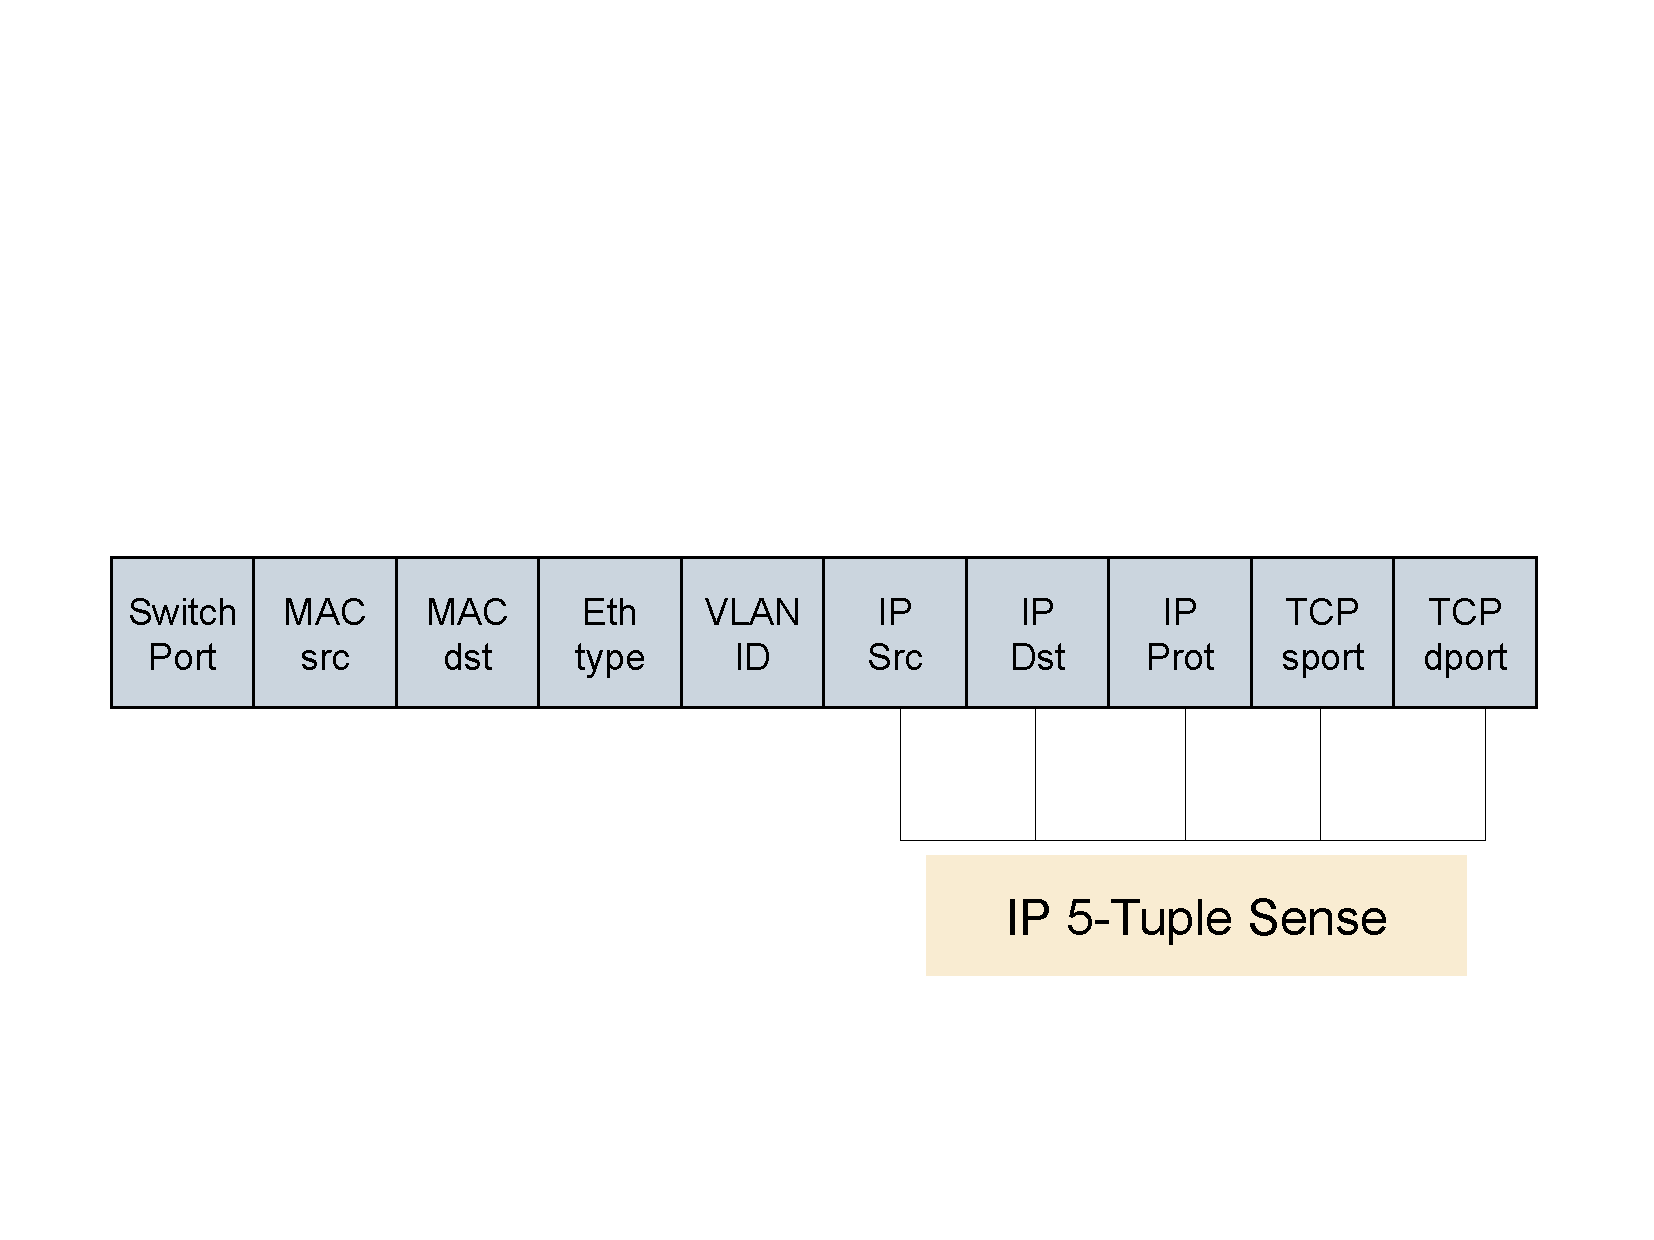
\includegraphics[height=1.5in, width=3.2in]{Pictures/10TUPLE.pdf}
	\caption{ OpenFlow \texttt{Ten-Tuple} format}
	\label{fig:tenTuple}
\end{figure}
\textbf{Flow Path Space} Upon testing the firewall on ODL controller and on a complicated topology, it was found that the IP-5 Tuple based approach is prone to ambiguous flow path calculations. An SND-Firewall with a centralized view of two or more different tenants, cannot successfully distinguish between tenants based solely on IP 5-Tuples. In a tenant based network like in datacenter, multiple disconnected tenants can be using similar network configurations. This will lead to hosts having identical IP 5-tuple addresses in two disconnected sub networks. On an OpenStack cloud with multiple different tenants, Flowguard produced conflicting flow path spaces and the comparison against the Firewall rules gave confusing resolutions. 
% Check for more concrete example, where with 5-tuple, firewall gives error.
In order to prevent the conflict, we propose to use a more fine grained, OpenFlow 10-Tuple sense Figure ~\ref{fig:tenTuple}. Apart from the existing fields in IP 5-Tuple sense, an OpenFlow 10-tuple also includes a physical layer-2  port, protocol type, VLAN-ID and Ethernet type. With this fine grained set of header fields, it is not possible to have duplicate route identification and thus we prevent the ambiguity in flow path space calculation. \\
\textbf{Firewall rule priority}
In a conventional firewall, priority of the rules are implicit based on their ordering. Provided a successful match, only higher priority firewall rule is considered for the action on traffic. In an SDN-firewall, the firewall rules and flow rules maintain their own set of priorities. SDN-Firewalls like FlowGuard divide the firewall rule space into two disjoint sets of \textit{allow} and \textit{deny} rules. These partitioning is however either done considering implicit rule priorities like in IP-tables or not considered at all. Thus, the firewall decision logic may violate the administrators intent of policy enforcement.
This can be fixed by taking the priorities of policies in account. However, this appears to be a difficult problem, as there are multiple sources like IDS, feedback module, firewall and network administrator who potentially install policies being ignorant of what higher priority conflicting rules exist in the network. It is still a problem even when their are no action-based conflicts between the rules, as redundant rules take unnecessary disk space on the controller. Duplicate rules are also a cause of performance degradation while checking for policy violations in the network. \\ \\
% Work on the dynamic priority decision algorithm
\textbf{Performance Issue}
The response time of FLOWGUARD substantially decreases as the network scales. This is because the conflict detection algorithm is based on dynamically propagating a sample flow in the logical snapshot of a network. Thus, when there are multiple actions per flow rule and many such flow rules as part of the flow path space, the propagation of a sample flow grows exponentially. When we tested the firewall on an convoluted topology of nodes and flow rules, the violation detection was in order of a few seconds. This window of time is good enough for an unauthorized communication to take place before a conflict is successfully resolved.
As a possible mitigation measure, we propose to maintain a reachability map which is updated during the initialization process of a firewall. Whenever there is an update, full propagation from source to destination can be avoided. Only partial propagation is required for only those edges in the plumbing graph which have undergone a change. For eg: If two hosts are connected via 5 switches in a linear topology. If a new flow rule update for the central switch in the path has been made, we do not need a propagation check from first node to the last for detecting violations. Instead, with the knowledge that 2/3 of the graph edge do not undergo a change, a propagation check can happen only for the last node. This saves time by reducing the propagation
time in proportion to the number of overlapping edges between the update and actual path.\\ \\
\textbf{Violation Resolution approaches}
Upon successful detection of flow and firewall policy violations, an SDN-Firewall should also be able to dynamically resolve the violations by either denying the new rules or modifying the existing flow tables. Different approaches have been proposed in FlowGuard to mitigate various kinds of violations. Many of these proposed approaches do their job of removing the violations but at the cost of availability and accuracy: deleted, modified and new rules prevent unauthorized traffic in the network by also end up denying communication between authorized hosts.
\subsubsection{Approach 1}
Dependency among flow rules having set-field actions can cause traffic to be matched by an unwanted flow rule. This can cause traffic steering among unauthorized hosts as mentioned in FlowGuard. An approach to break the inter-dependency is by tagging the header fields. Match fields in flow rules are tagged to break any violating dependencies. This is however achieved at the cost of losing the critical information of the flow field which is tagged. For eg., in FlowGuard, vlan-tagging is used wherein VLAN field in flow rule is tagged to break its dependency from another flow rule in same or different switch. In our testing in multi tenant networks, VLAN field plays a significant role in traffic steering between different subnets. Thus, by tagging VLAN field with a hard coded value, the dependency can be broken but the flow rules intended purpose to match on VLAN field is also lost. Any flow which is not part of dependency process but is using the tagged field to process the packet further in the network, fail to match the traffic in which packet headers are now changed. 
\subsubsection{Approach 2}
When a firewall detects there is entire violation in the existing flow path, all the rules present in the flow path are removed from the corresponding switches on the network\cite{FLOWGUARD}. Only tracked path comprising of source address from the incoming packets and destination address from the outgoing packet is matched against the Firewall rule policies. In our testing we found that this approach might leave the network disconnected if the  \textit{tracked flow path space} encompasses more than two switches or flow tables. For eg., if a violating tracked space consists of rules from 5 different switches and one of the rules in a third switch(middle node) is a wildcarded rule allowing this "unauthorized" communication, all the rules including the wildcared one are deemed unnecessary and removed. This leads to denial of any authorized communication also that the wildcarded rule was allowing in the network.
% Give the example in diagram
To prevent such complex resolutions from being too harsh on the network, higher priority rules with finer granularity should rather be installed. The wildcarded flows require special attention as they are responsible for both allowed and denied traffic through them.
\subsubsection{Approach 3}
Another issue with removing a flow from a network is that with new Openflow protocol, the actions per match in one flow rule can be chained. This means, when a flow in network is matched by a flow rule in a switch, the same packet can undergo multiple actions, which include output to a physical port of that switch, send to controller or \textit{drop}. Upon detecting a violation in a flow rule, deleting the entire flow rule, deletes all the violating and non violating actions within it. This means the deletion of a flow rule requires carefully examination. The action set within a rule can only partially violate the policy just like entire flow rule can have partial violations.\\
\textbf{Disregard for concurrent updates}
In our testing we have found issues when multiple user threads or applications make concurrent updates on firewall policy or flow policy. In case of conflicting updates, lack of handling the concurrency leads to low priority rule with a different action on same match being handled before the higher priority rule. For eg. if an admin uses REST call to install a new flow rule in the network but a countermeasure engine at the same time install a conflicting action on the same match as by REST call, the decision of unsynchronized firewall depends on which thread is executed before. The issue with concurrent updates becomes a problem when firewall applications are deployed in an enterprise networks where there are multiple pipelines which update the same flow policy data stores.
\begin{comment}
\section{Advanced SDN-Firewall functions}
Attacks in a complex network like datacenters can originate from external world and from within. As mentioned before, the SDN-firewall cannot trust the traffic and hosts present inside the network just like it treats outside world. With abstraction in SDN, different attacks target separate layers \cite{SECSDN}. The SDN-Firewall should protect the controller and network against the attacks originating from northbound applications and also from network. Using the pool of information provided by OpenFlow protocol and SDN control plane, an SDN-Firewall potentially can provide multi dimension protection instead of just being a ACL policy enforcer. We have identified new attack vectors in an SDN environment and prevention measures that should be included in an SDN-based Firewall. As part of future work in the same direction, we are identifying different vulnerabilities in the industry accepted controllers. - OpenDayLight and ONOS.
\begin{enumerate*}
	\item \textit{Denial of Service}\item \textit{Flow Flooding}\item \textit{Memory Exhaustion}
	\item \textit{Link Saturation}
	\item \textit{CPU Exhaustion}
	\item \textit{Switch Spoofing}
\end{enumerate*}
\end{comment}

\section{Conclusion and Future Work}

In this work we have juxtaposed existing SDN-based firewalls to inspect their readiness to be deployed in enterprise and large scale networks. We have identified various metrics that an SDN based firewall solution should adhere to. Seven different firewalls meant for different SDN controllers are compared and evaluated against the metrics. As a special case, we have deployed FlowGuard\cite{FLOWGUARD} on OpenDayLight controller and discovered vulnerabilities when the capabilities are scaled to a complex network. These vulnerabilities are individually discussed and possible mitigation measures are proposed. With abstraction in SDN, different attacks target separate layers \cite{SECSDN}. The SDN-Firewall should protect the controller and network against the attacks originating from northbound applications and also from network. As a part of our future work in the same direction, we intend to identify different vulnerabilities in the industry accepted controllers - OpenDayLight and ONOS: 
 \begin{enumerate*}
 	\item \textit{Denial of Service}\item \textit{Flow Flooding}\item \textit{Memory Exhaustion}
 	\item \textit{Link Saturation}
 	\item \textit{CPU Exhaustion}
 	\item \textit{Switch Spoofing}
 \end{enumerate*}
 
\begin{acks}
	This research is based upon work supported by the National Science Foundation towards Secure and Resilient Architecture: SciGuard project under Grant \grantnum{1528099}.
\end{acks}
